\begin{frame}{Bloch sphere}
\begin{itemize}
    \item<1-> Visualize single qubit transformations
    \item<2-> \code{kaleidoscope} library
    \item<3-> input \(=\) vector representing the quantum state
    \item<4-> interactive!
\end{itemize}

\begin{center}
    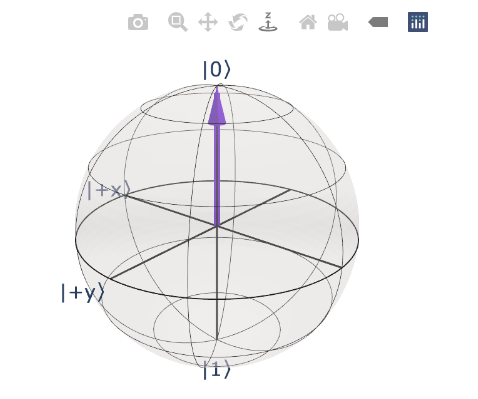
\includegraphics[width=0.5\textwidth]{img/lec1/bloch_sphere.png}
\end{center}
\end{frame}

\begin{frame}[fragile]{The code (6)}
\begin{minted}{python}
!pip install kaleidoscope
from kaleidoscope import bloch_sphere
from qiskit.quantum_info import Statevector
qc = QuantumCircuit(1)
figure = bloch_sphere(Statevector.from_instruction(qc))
figure.show()
\end{minted}
\end{frame}

% https://github.com/Qiskit/qiskit-tutorials/blob/master/tutorials/circuits_advanced/01_advanced_circuits.ipynb